\title{Non--Archimedean Geometry}
\author{\textit{Based on a lecture series by }Enrica Mazzon.}
\date{December 2024}
\maketitle

Introduction to non--Archimedean geometry and applications of the
techniques to algebraic geometry.

\subsection{About} This course on pseudolattices was a part of a Winter
School for students and early career researchers, organised by the UK Algebraic
Geometry Network. The lectures were delivered in-person in the University of
Warwick, and were transcribed by Parth Shimpi. These notes have undergone
several amendments and are not a verbatim recall of the lectures, therefore
discretion is advised when using this material. They are available online at
\url{https://pas201.user.srcf.net/documents/2023-ukag-pseudolattices.pdf}.
All errors and corrections should be communicated to by email to
\url{parth.shimpi@glasgow.ac.uk}.

\section{Non--Archimedean fields}
Let \(\bbF\) be a field. A \emph{semi-norm} is a map \(|\cdot|:\bbF\to
\mathbb{R}_{\geq 0}\) such that \(|0|=0\), \(|1|=1\), \(|a+b|\leq |a|+|b|\), and
\(|ab|\leq |a|\cdot |b|\). If moreover we require that \(|ab|=|a|\cdot |b|\),
then the seminorm is \emph{multiplicative}. If \(|a|>0\) whenever \(a\neq 0\), then \(|\cdot |\) is called a \emph{norm}.

A semi-norm \(|\cdot |\) is non--Archimedean if it satisfies the strong triangle
inequality \(|a+b|\leq \max\{|a|,|b|\}\).

\begin{remark}
If \(|\cdot|:\bbF\to \mathbb{R}_{\geq 0}\) is a non--Archimedean multiplicative
norm, then \(v(-)=-\log |\cdot |\) is a non--Archimedean valuation.
\end{remark}

We say \((K,|\cdot|)\) is a non--Archimedean field if it is a field endowed with
a non--Archimedean multiplicative norm. In this case, we say \(R=K^0=\{x\in
K\;|\; |x|\leq 1\}\) is the \emph{valuation ring},
\(K^\infty=\mathfrak{m}=\{x\in K\;|\; |x|<1\}\) is the maximal ideal, and
\(\tilde K = R/\mathfrak{m}\) is the residue field of \(K\).

\begin{example}
Any field \(\bbF\) can be endowed with the trivial norm \(|\cdot|_0\) defined as
\(|0|_0=0, |a|_0=1\). Then \(\bbF=\bbF^0=\tilde\bbF\) and \(\bbF^\infty = \{0\}\).
\end{example}

\begin{example}
If \(\bbF\) is any field, then we can consider the associated field of Laurent series
\[K=\bbF ((t)) = \{\sum_{i=N}^\infty a_i t^i \text{ for some
}N\in\mathbb{Z}, a_i\in \bbF\}.\] Then any \(\varepsilon\in (0,1)\) determines a
norm \(|0|=0\), \(|f|=\varepsilon^{\text{ord}_t(f)}\). Then \(K^0=\bbF\llbracket t
\rrbracket\), \(K^\infty = (t)\), \(\tilde K = \bbF\).
\end{example}

\begin{example}
The field of \(p\)-adic rationals \[\mathbb{Q}_p=\{\sum_{i=N}^\infty a_i p^i
\text{ for some }N\in\mathbb{Z}, a_i\in \{0,...,p-1\}\}.\] Again, any
\(\varepsilon\in (0,1)\) determines a norm \(|s|=p^{-\text{ord}_p(s)}\). It is
customary to take \(\varepsilon=\frac{1}{p}\) in number theory. Have
\(\mathbb{Q}_p^0=\mathbb{Z}_p\), \(\mathbb{Q}_p^\infty =(p)\),
\(\widetilde{\mathbb{Q}_p} = \mathbb{F}_p\).
\end{example}

\begin{remark}
    A norm \(|\cdot|\) is Archimedean if it satisfies the Archimedean property,
    i.e.\ for every \(r\in\mathbb{R}_{\geq 0}\) there exists an \(n\in
    \mathbb{Z}\) with \(|n|\geq r\). Show that a norm is non--Archimedean if and
    only if \(|\cdot|\) is uniformly defined on the image of \(\mathbb{Z}\to
    K\).
\end{remark}

\subsection{Motivation for non--Archimedean fields in algebraic geometry} Say
you wish to understand the geometry of a smooth projective
\(\mathbb{C}\)--variety \(X\). A possible technique is to place \(X\) in a
\(1\)--parameter family \(f:\mathscr{X}\to \mathbb{A}^1=\Spec(\mathbb{C}[t])\)
i.e.\ \(\mathscr{X}_1=f^{-1}(1)\cong X\) and \(\mathscr{X}_0=f^{-1}(0)\) (a \emph{degeneration}) is a union
of irreducible components with simpler structure, thus turning some of the
geometric complexity combinatorial.

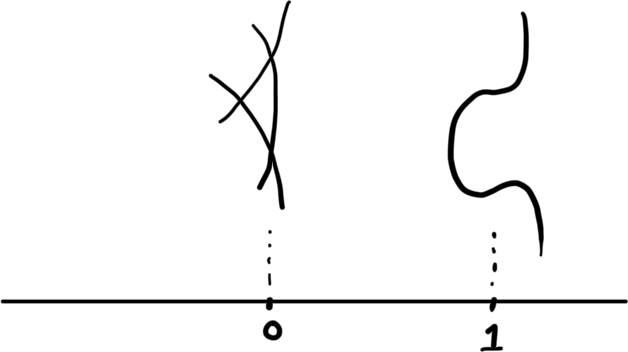
\includegraphics[width=0.5\textwidth]{images/degeneration-eg.png}

Then we consider the base change of \(\mathscr{X}\) to a infinitesimal punctured
tubular neighbourhood of \(\mathscr{X}_0\), to obtain
\(\mathscr{X}\times_{\mathbb{C}[t]}\Spec(\mathbb{C}((t)))\). This is a variety
over \(K=\mathbb{C}((t))\).

\(K\)--analytic manifolds. Over \(\mathbb{C}\) with usual norm, a smooth
algebraic variety \(X\) is locally defined by polynomials \(f_1,...,f_m\in
\mathbb{C}[x_1,...,x_n]\). One can turn \(X\) into a complex manifold
\(X(\mathbb{C})\), by locally considering the subset \(\{(x_1,...,x_n)\in
\mathbb{C}^n\;|\; f_i(x_1,...,x_n)=0\}\) with the geometry inherited from
\(\mathbb{C}^n\). This allows us to apply new techniques (complex analysis,
differential geometry, Hodge theory, etc) to study \(X\). When \(X\) is proper,
this process of analytification incurs no loss of information in the sense of
Serre's GAGA theorem-- two smooth proper \(\mathbb{C}\)--varieties \(X,Y\) are
isomorphic if and only if \(X(\mathbb{C})\cong Y(\mathbb{C})\) as complex
manifolds.

What's the topology on \(X(\mathbb{C})\)? It is the weakest topology such that
for any Zariski--open set \(U\subset X\), the subset \(U(\mathbb{C})\subset
X(\mathbb{C})\) is open and for any regular function \(f\in \OO_X(U)\) the map
\(|f|:U(\mathbb{C})\to \mathbb{R}\) is continuous.

What's the sheaf of functions? We consider \emph{analytic functions}, on an open
set \(V\subset X(\mathbb{C})\) these are those that can be written locally as a
uniform limit of regular functions. Then
\(X^\text{an}=(X(\mathbb{C}),\OO_{X(\mathbb{C})})\) is a complex manifold.

When \(K\) is a non--Archimedean field, the na\"ive idea is to replicate the
same construction. However, the analogue of the GAGA principle fails in a
spectacular way. To see this, given \(a\in K, r\in \mathbb{R}_{\geq 0}\) write
\(B^+(a,r), B^-(a,r)\) for the closed and open balls of radius \(r\) centered at
\(a\) respectively. In the trivially valued case, \(B^+(a,1)=K\),
\(B^+(a,\frac{1}{2}) = a\). In particular the metric topology on \(K\) is
discrete. In the non--trivially valued case, consider \(r'\leq r\) and suppose
\(B^+(0,r)\cap B^+(a,r')\) is non--empty. Then in fact \(B^+(a,r')\subseteq
B^+(0,r)\), i.e.\ closed balls are either disjoint or nested.
Exercise: every point in a ball is a center of the ball. Exercise: every ball in
\(K\) is both open and closed in the metric topology. Thus the metric topology
is totally disconnected, i.e.\ the only connected subsets have cardinality
\(\leq 1\).

Issues: the characteristic (indicator) function of a ball is continous and
analytic. There are too many analytic functions, and thus too many analytic
isomorphisms. Thus have the `death of GAGA': Serre proved every
\(n\)--dimensional \(\mathbb{Q}_p\)--analytic manifold in this na\"ive sense is
isomorphic to a disjoint union of up to \(p-1\) copies of \(B^+(0,1)^n\).

\section{Berkovich spaces}
In the 90s, Berkovich adopted the philosophy that the topology of the
\(K\)--analytification is itself not a problem; rather there are many points
that are missing from the definition of a \(K\)--analytic manifold. The
resulting theory becomes very close to the that of \(\mathbb{R}\) and
\(\mathbb{C}\)--manifolds.

\begin{definition}
    Let \(K\) be a complete non--archimedean field, and \(X\) a \(K\)--variety.
    We set \[X\an=\{x\in (\zeta_x, |\cdot|_x)\;|\; \zeta_x \text{ is a point of
    \(X\)}, \quad |\cdot|_x \text{ is a multiplicative norm on the residue
    field \(k(\zeta_x)\) extending \(|\cdot|\) on \(K\)}\}\]
\end{definition}

\begin{remark}
If \(\zeta_x\) is a closed point then \(k(\zeta_x)\) is a finite extension of
\(K\) and thus there is a unique \(|\cdot|_x\). Thus \(X(K)\) is a subset of
\(X\an\).

If \(\zeta_x\) is not a closed point then the extension \(k(\zeta_x)/K\) is
transcendental and thus there are infinitely many ways to extend the seminorm.
This forms the `main' part of \(X\an\).
\end{remark}

We endow \(X\an\) with the weakest topology such that the forgetful map \(i:X\an
\to X\) is continuous, and for all open \(U\subset X\) and for all \(f\in
\OO_X(U)\), the map \(i^{-1}(U)\to \mathbb{R}\) given by
\((\zeta_x,|\cdot|_x)\mapsto |f(\zeta_x)|_x\) is continuous.

The sheaf of analytic functions comes by assigning every open set \(V\subset
X\an\) to the set of functions thhat are locally a uniform limit of regular
functions.

\subsection{Properties}
\begin{enumerate}[start=0]
\item Taking \(K=\mathbb{C}\) with the usual norm gives the usual complex
manifold \(X(\mathbb{C})\)-- this is because the only valued extension of
\(\mathbb{C}\) is trivial so the non--closed points are not a part of \(X\an\).

\item \(X\an\) is locally  compact and locally path connected. Moreover, \(X\)
is connected (separated, proper) if and only if \(X\an\) is connected (resp.\
Hausdorff, compact).

(Howshovski--Loeser) show that \(X\an\) is locally contractible and has the
homotopy type of a polyhedron.

\item GAGA--type results hold, and there is an equivalence between proper
algebraic \(K\)--varieties and their analytifications.
\end{enumerate}

\begin{example}
If \(X=\Spec A\) is affine for some \(K\)--algebra \(A\), then the set \(X\an\)
can be described as the set of all multiplicative seminorms \(|\cdot |_x:A\to
\mathbb{R}_{\geq 0}\) extending \(|\cdot|\). The topology is then the weakest
such that \(|f|:X\an\to \mathbb{R}\) is continuous for all \(f\in A\).
\end{example}

\begin{example}[The Berkovich line]
Consider \(X=\mathbb{A}^1_K=\Spec K[y]\), and suppose \(K\) is an algebraically
closed complete non--Archimedean field.

If \(K\) is equipped with the trivial norm \(|\cdot|_0\), then a point \(x\in X\an\)
corresponds to multiplicative seminorms \(|\cdot|_x:k[y]\to \mathbb{R}_{\geq
0}\) extending the trivial norm. Since \(K\) is algebraically closed, it
suffices to describe such a seminorm on linear polynomials of the form
\((y-a)\). One such norm is the `Gauss norm' \(\eta_{\text{Gauss}}\), which is
simply the trivial norm \(\eta_\text{Gauss}(y-a)=1\) for all \(a\in K\).

Every \(a\in K\) defines a seminorm \(\eta_{a,0}:K[y]\to \mathbb{R}\)
given by \(f\mapsto |f(a)|_0\), i.e.\ \(\eta_{a,0}(y-b)=|a-b|_0 = 1\) if \(b\neq a\)
and \(\eta_{a,0}(y-a)=0\).

On the other hand, every \(a\in K\) and \(r\in (0,1)\) defines a seminorm
\(\eta_{a,r}\) given by \(f\mapsto r^{\text{ord}_a(f)}\). Thus
\(\eta_{a,r}(y-a)=r\) and \(\eta_{a,r}(y-b)=1\) if \(b\neq a\). In the limit
\(r\to 0\) this recovers \(\eta_{a,0}\), and in the limit \(r\to 1\) this
recovers \(\eta_\text{Gauss}\).

For \(r\in (1,\infty)\), we can also define the seminorm \(\eta_{\infty ,r}\)
given by \(f\mapsto r^{\deg(f)}\). In the limit \(r\to 1\) this again recovers
\(\eta_\text{Gauss}\).

These are all the points of \(X\an\) which can be pictorially represented as
follows.

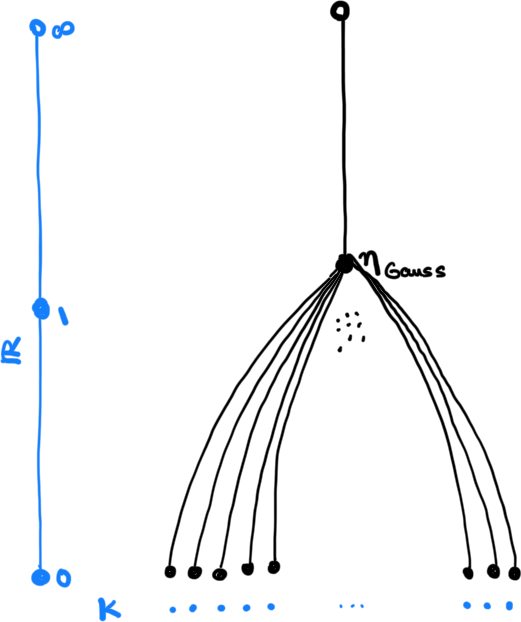
\includegraphics[width=0.5\textwidth]{images/birkovich-line.png}

To describe the topology, consider the polynomial \(f=y\). The open sets
determined by this are \(U_{s<s'}=\{x\in X\an\;|\; s< |y|_x < s'\}\) for
\(s<s'\) in \(\mathbb{R}\). If \(s'<1\) then this is \(\bigcup_{a\in
K}\{\eta_{a,r}\;|\; r\in (s,s')\}\). If \(s>1\) then \(\{\eta_{\infty,r}\;|\;
r\in (s,s')\}\). If \(s<1\) and \(s'>1\) then ...

Thus the topology is the metric topology on legs \([0,1)\) and \((1,\infty)\),
while any open neighbourhood of \(\eta_\text{Gauss}\) contains all but finitely
many legs.

\textbf{If \(K\) is algebraically closed and non--trivially valued} The points
\(\eta_{a,0}:f\mapsto |f(a)|\) can still be defined. On the other hand for
\(a\in K\) and \(r>0\), we can define \(\eta_{a,r}\) by \(f\mapsto \sup_{z\in
B^+(a,r)} |f(z)|\). If \(r\geq |a|_K\), then \(B^+(a,r)=B^+(0,r)\) and so
\(\eta_{a,r}=\eta_{0,r}\) for \(r\) sufficiently large. More generally,
\(\eta_{b,r}=\eta_{c,r}\) for \(r\geq|b-c|\). This gives an infinite tree
branching at every value of \(K\). The points correspond to open
balls in \(K\) or sequences of nested balls. It is possible for an infinite
intersection of nested balls to be empty.

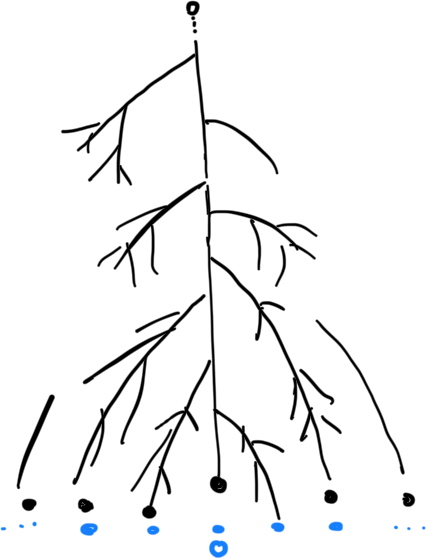
\includegraphics[width=0.5\textwidth]{images/birkovich-line-2.png}

The topology is such that any open neighbourhood of a branching point contains
all but finitely many branches.

\end{example}

If \(K,|\cdot |\) is a non--Archimedean field, then taking \(-\log|\cdot |\)
gives a non--Archimedean \emph{valuation} \(v:K\to \overline{\mathbb{R}} = \mathbb{R}\cup \{\infty\}\), i.e.\ a valuation such that \(v(a+b)\geq
\min\{v(a),v(b)\}\).

Let \(K\) be algebraically closed and non--trivially valued. The
\emph{tropicalisation map} of \(\mathbb{A}^n_K\) is defined as
\(\text{trop}:\mathbb{A}^n_K(K)\to \overline{\mathbb{R}}^n\) given by
\((x_1,...,x_n)\mapsto (v(x_1),...,v(x_n))\), and extend it to the Birkovich
analytification by \(((y_1,...,y_n),v_x)\mapsto (v_x(y_1),...,v_x(y_n))\).

The \emph{tropicalisation} of \(\mathbb{A}^n_K\) is the closure of
\(\text{trop}(\mathbb{A}^n_K(K))\) which is equal to
\(\text{trop}(\mathbb{A}_K^n\an)\).

For \(X\subseteq \mathbb{A}^n_K\), can define tropicalisation by restriction,
but this actually depends on the embedding of \(X\) into \(\mathbb{A}^n_K\).

\begin{example}
    Fix \(X=\mathbb{A}^1_K=\Spec K[y]\).

    \begin{enumerate}
        \item if we take the trivial inclusion \(\text{id}:\mathbb{A}^1_K\to
        \mathbb{A}^1_K\), then the tropicalisation with respect to this
        inclusion sends a seminorm \(\eta\in\mathbb{A}^1_K\an\) to \(-\log
        \eta(y)\). Thus \(\text{trop}(\eta_{0,0})=\infty\),
        \(\text{trop}(\eta_{0,r})=-\log(r)\), while
        \(\text{trop}(\eta(a,r))=-\log |a|\) whenever \(r<|a|\). Every branch
        gets `contracted back to branch point'.

        \item On the other hand consider the inclusion \(\mathbb{A}^1_K\into
        \mathbb{A}^2_K\) by \(y\mapsto (y+t, y-t)\), so that \(\eta\) maps to
        \((\log \eta(y+t), \log\eta(y-t))\).

        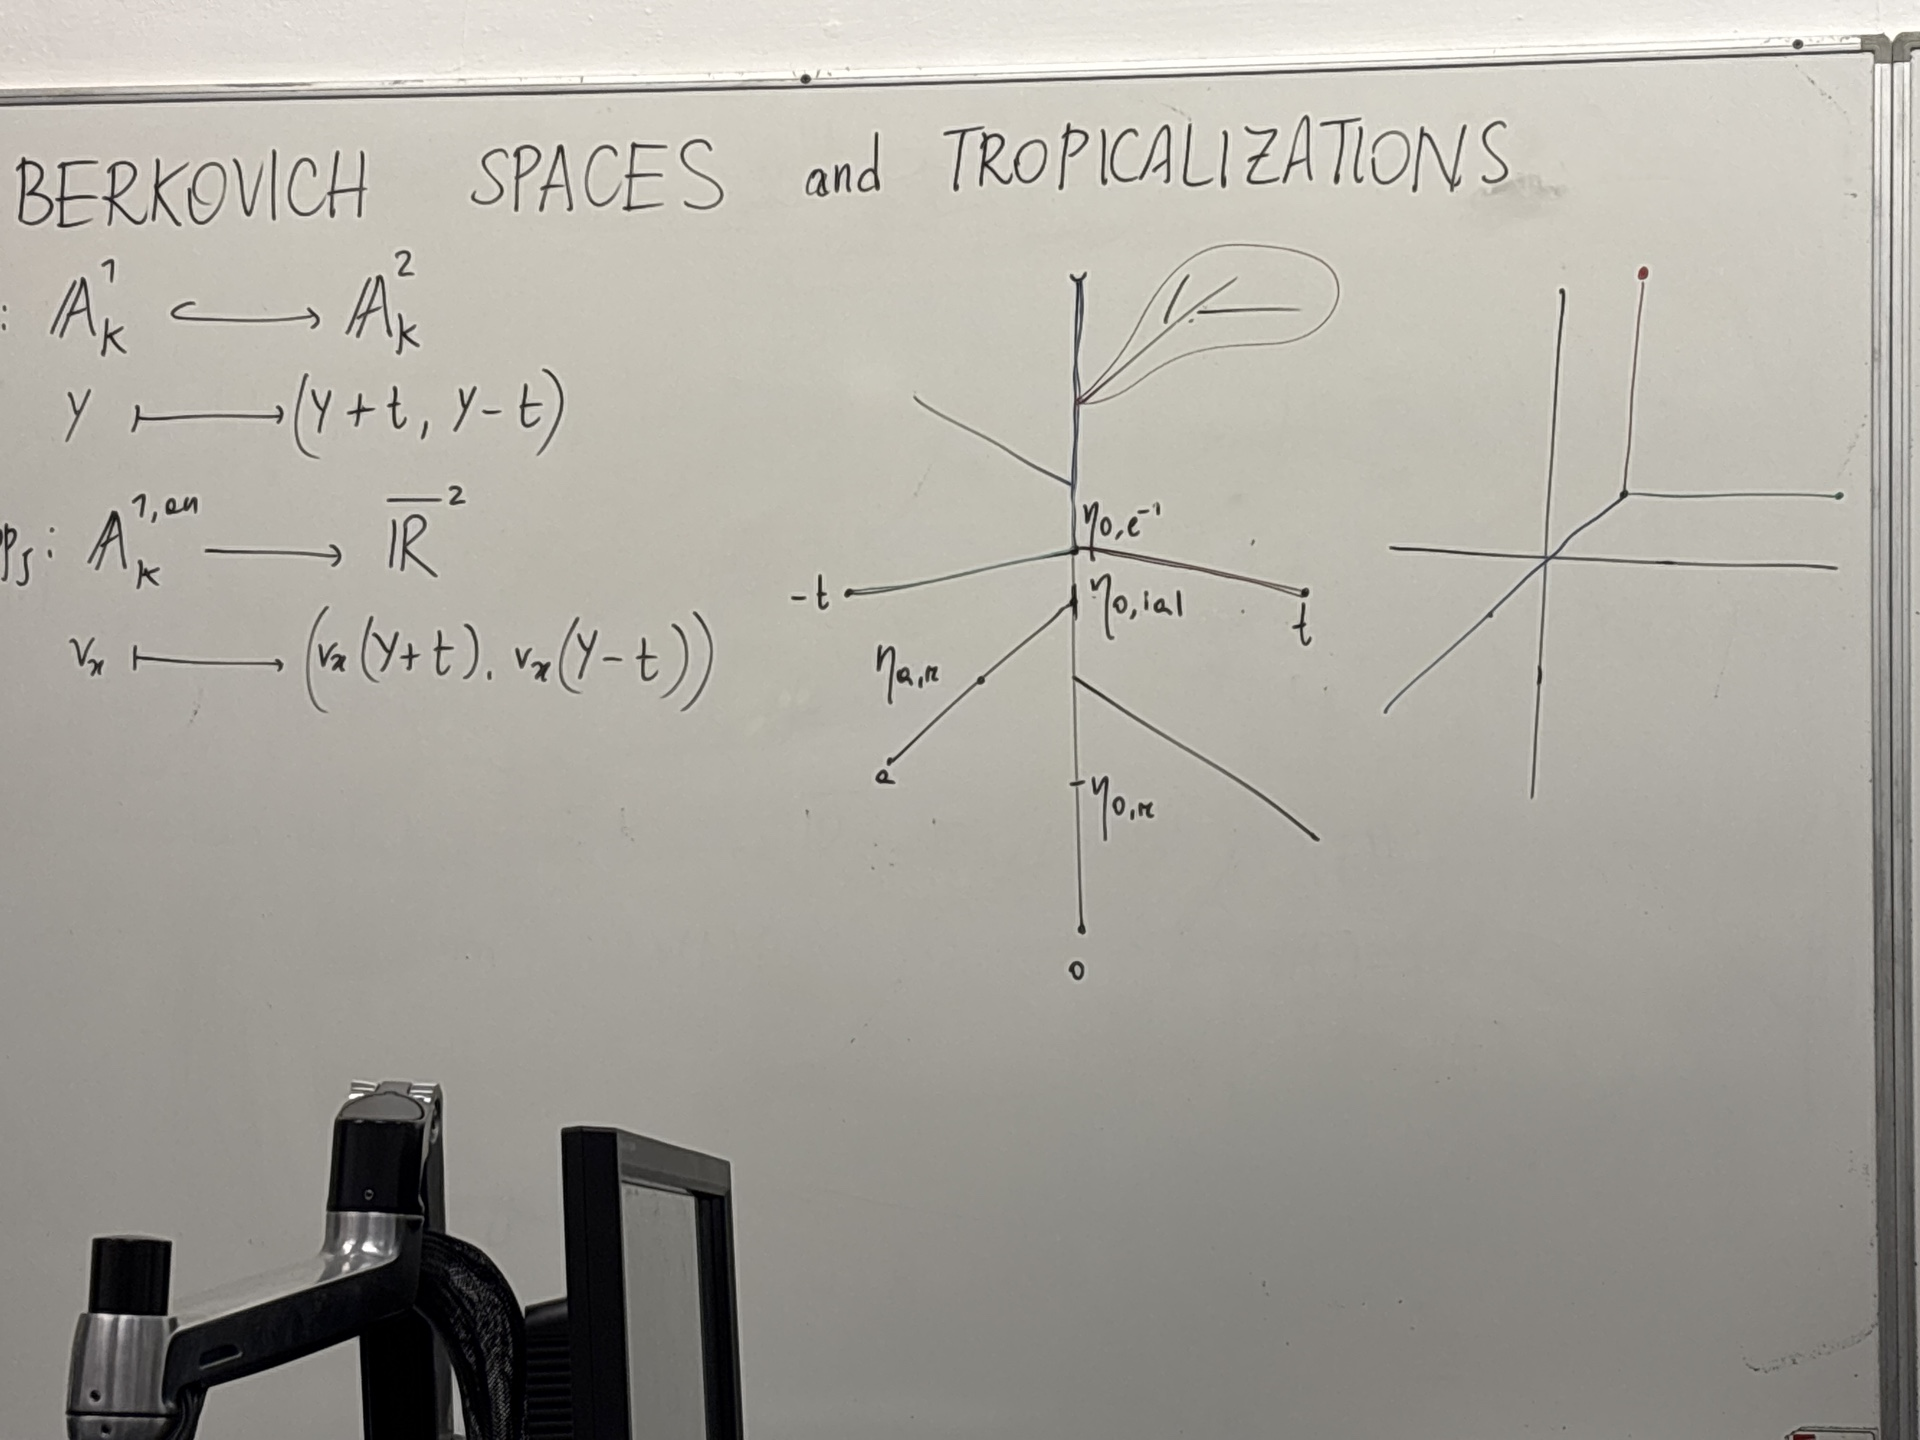
\includegraphics[width=0.5\textwidth]{images/A1-embedding.jpeg}

        \item If we take the inclusion \((y+t,y-t,y+1-t)\) in \(\mathbb{A}^3\),
        get similar picture, with two trivalent vertices and four infinite arms.


        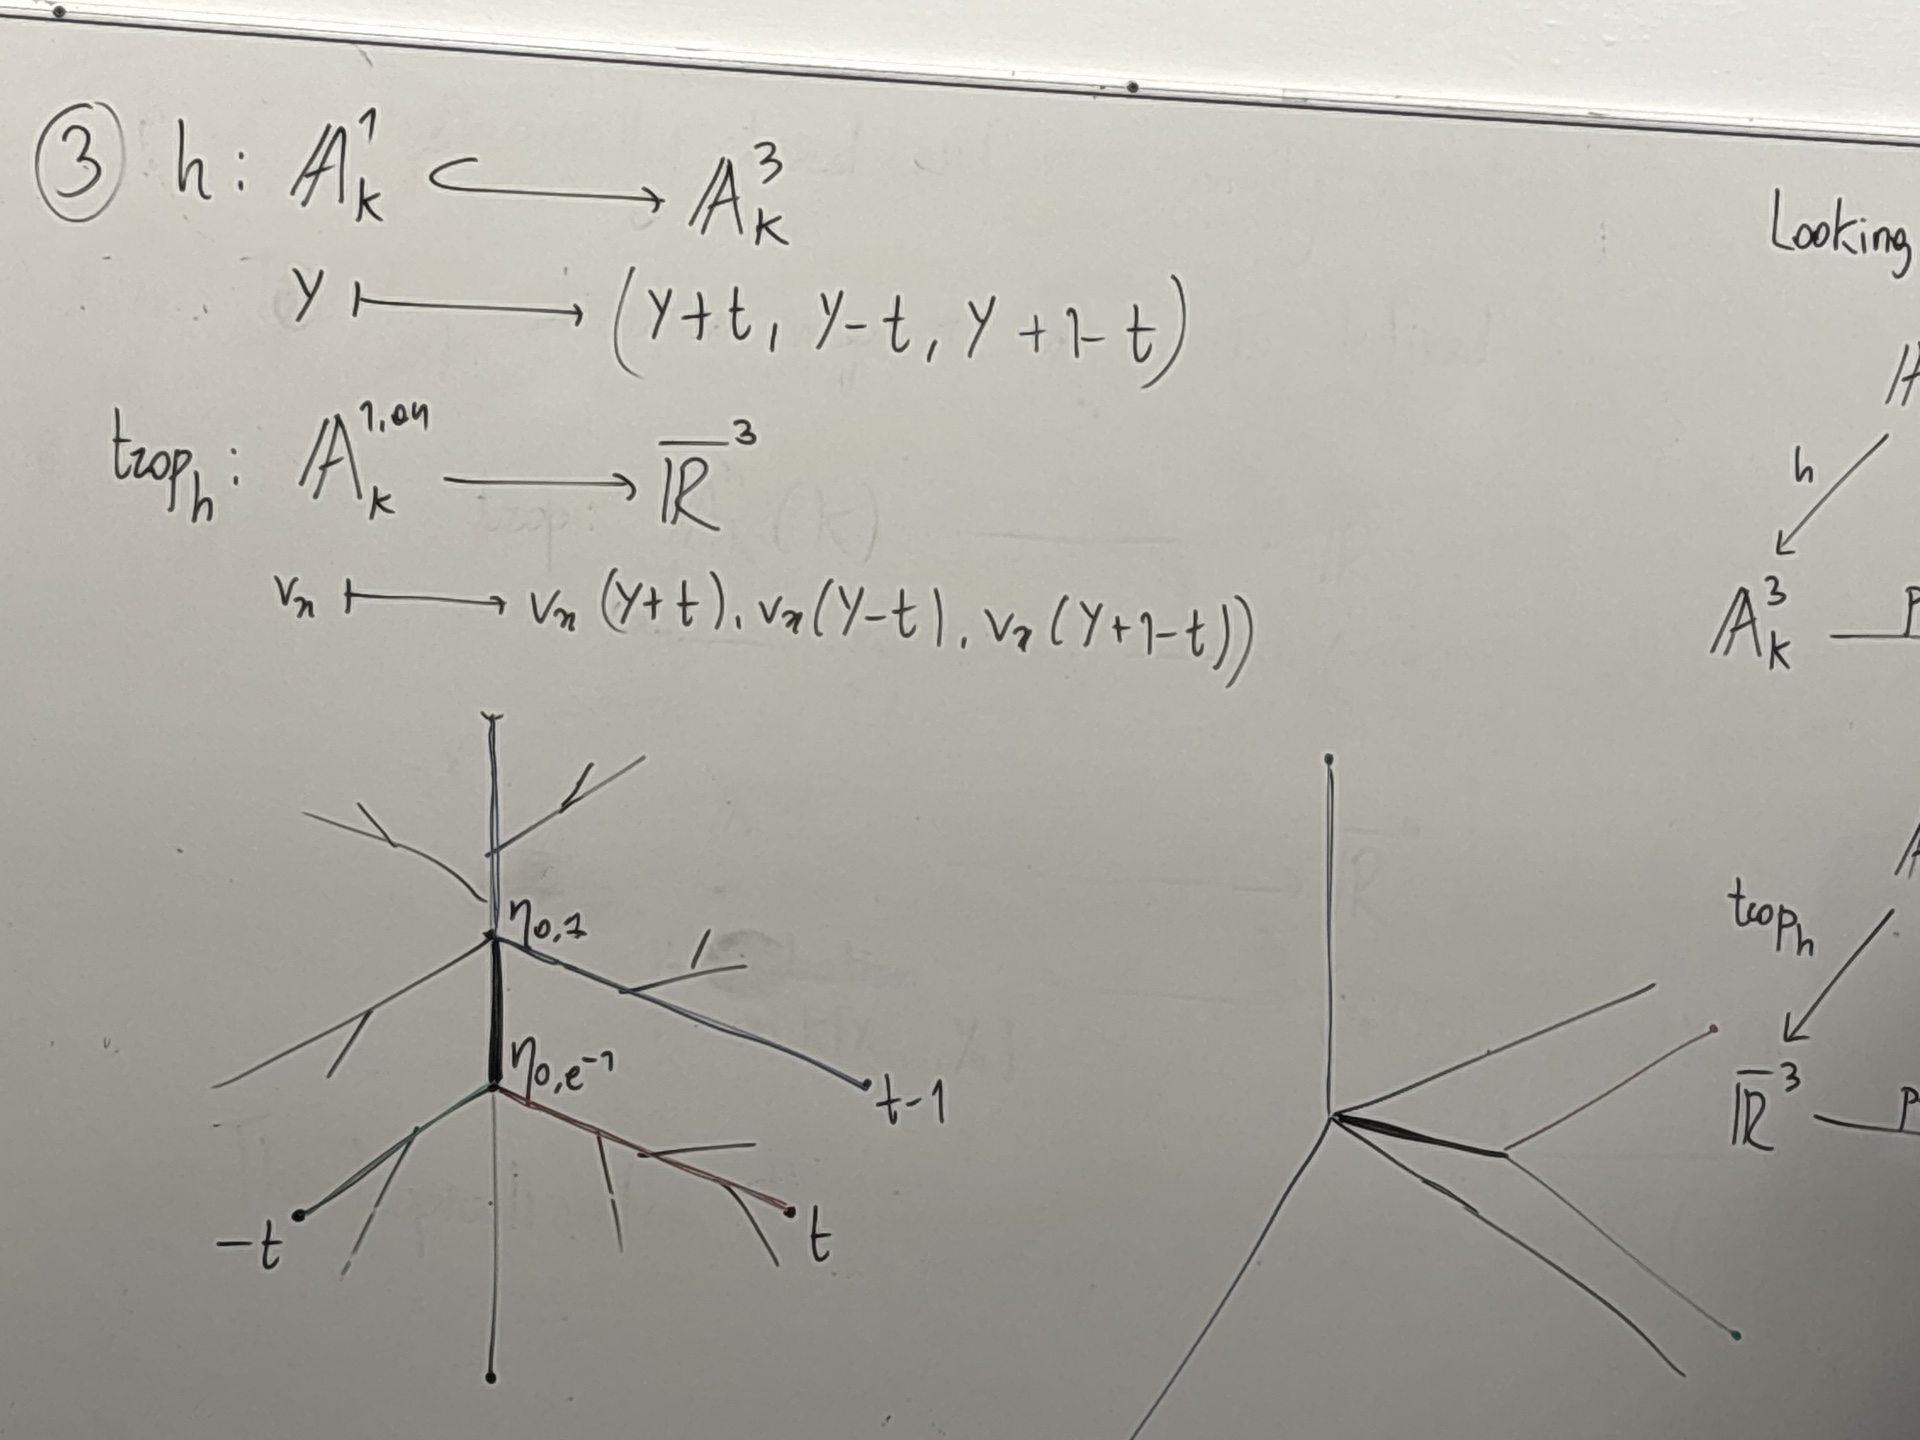
\includegraphics[width=0.5\textwidth]{images/A1-embedding-A3.jpeg}
    \end{enumerate}
\end{example}

Observe that tropicalisation 3 projects onto tropicalisation 2.

\begin{theorem}[(Payne)]
For \(K\) algebraically closed and non--trivially valued, with \(X\) a closed
subvariety of \(\mathbb{A}^n/\mathbb{P}^n/\)some torc variety, taking the inverse limit of
\(\text{Trop}(X,i)\) over all inclusions \(i\) is homeomorphic to \(X\an\).
\end{theorem}

\section{Dual complexes}
Consider the non--Archimedean field \(K=\mathbb{C}(\!(t)\!)\), then a
\(K\)--variety is a family of varieties parametrised over \(t\neq 0\) [IMAGE OF CONIC FAMILY XY=T]

Writing \(R=\mathbb{C}[\![t]\!]\) for the valuation ring, we say a degeneration
of the family over \(t=0\) is an snc model \(\mathcal{X}\) of \(X\) over \(R\)
where we require the special fiber \(\mathcal{X}_0\) to be a snc divisor with
smooth components. To this we associate a \emph{dual complex} where each
component of \(\mathcal{X}_0\) is a vertex, and there is a \(k\)--simplex
\([D_1,D_2,...,D_k]\) for every irreducible non--empty component of \(D_1\cap
D_2\cap...\cap D_k\).

The dual complex of \(\mathcal{X}_0\) embeds into \(X\an\), i.e.\ for every
point of the dual complex we can associate a valuation of \(K[x,y]/(xy-t)\). The
point associated to the point \(\alpha\in D_1\bullet - \bullet D_2 \cong [0,1]\) corresponds to valuation \(v_\alpha(x)=1-\alpha, v_\alpha(y)=\alpha\).

\begin{proposition}
Let \(X\) be a smooth proper vareity over \(K=\mathbb{C}((t))\). Then for any
snc model \(\mathcal{X}\) of \(X\) over \(R=\mathbb{C}[[t]]\), the dual complex
of \(\mathcal{X}_0\) embeds into \(X\an\). We say the image \(Sk(\mathcal{X})\)
is the skeleton. Further, \(X\an\) retracts onto this skeleton and this is
actualy a strong deformation retraction.

Taking the inverse limit over all snc models recovers the Birkovich
analytification \(X\an\).
\end{proposition}

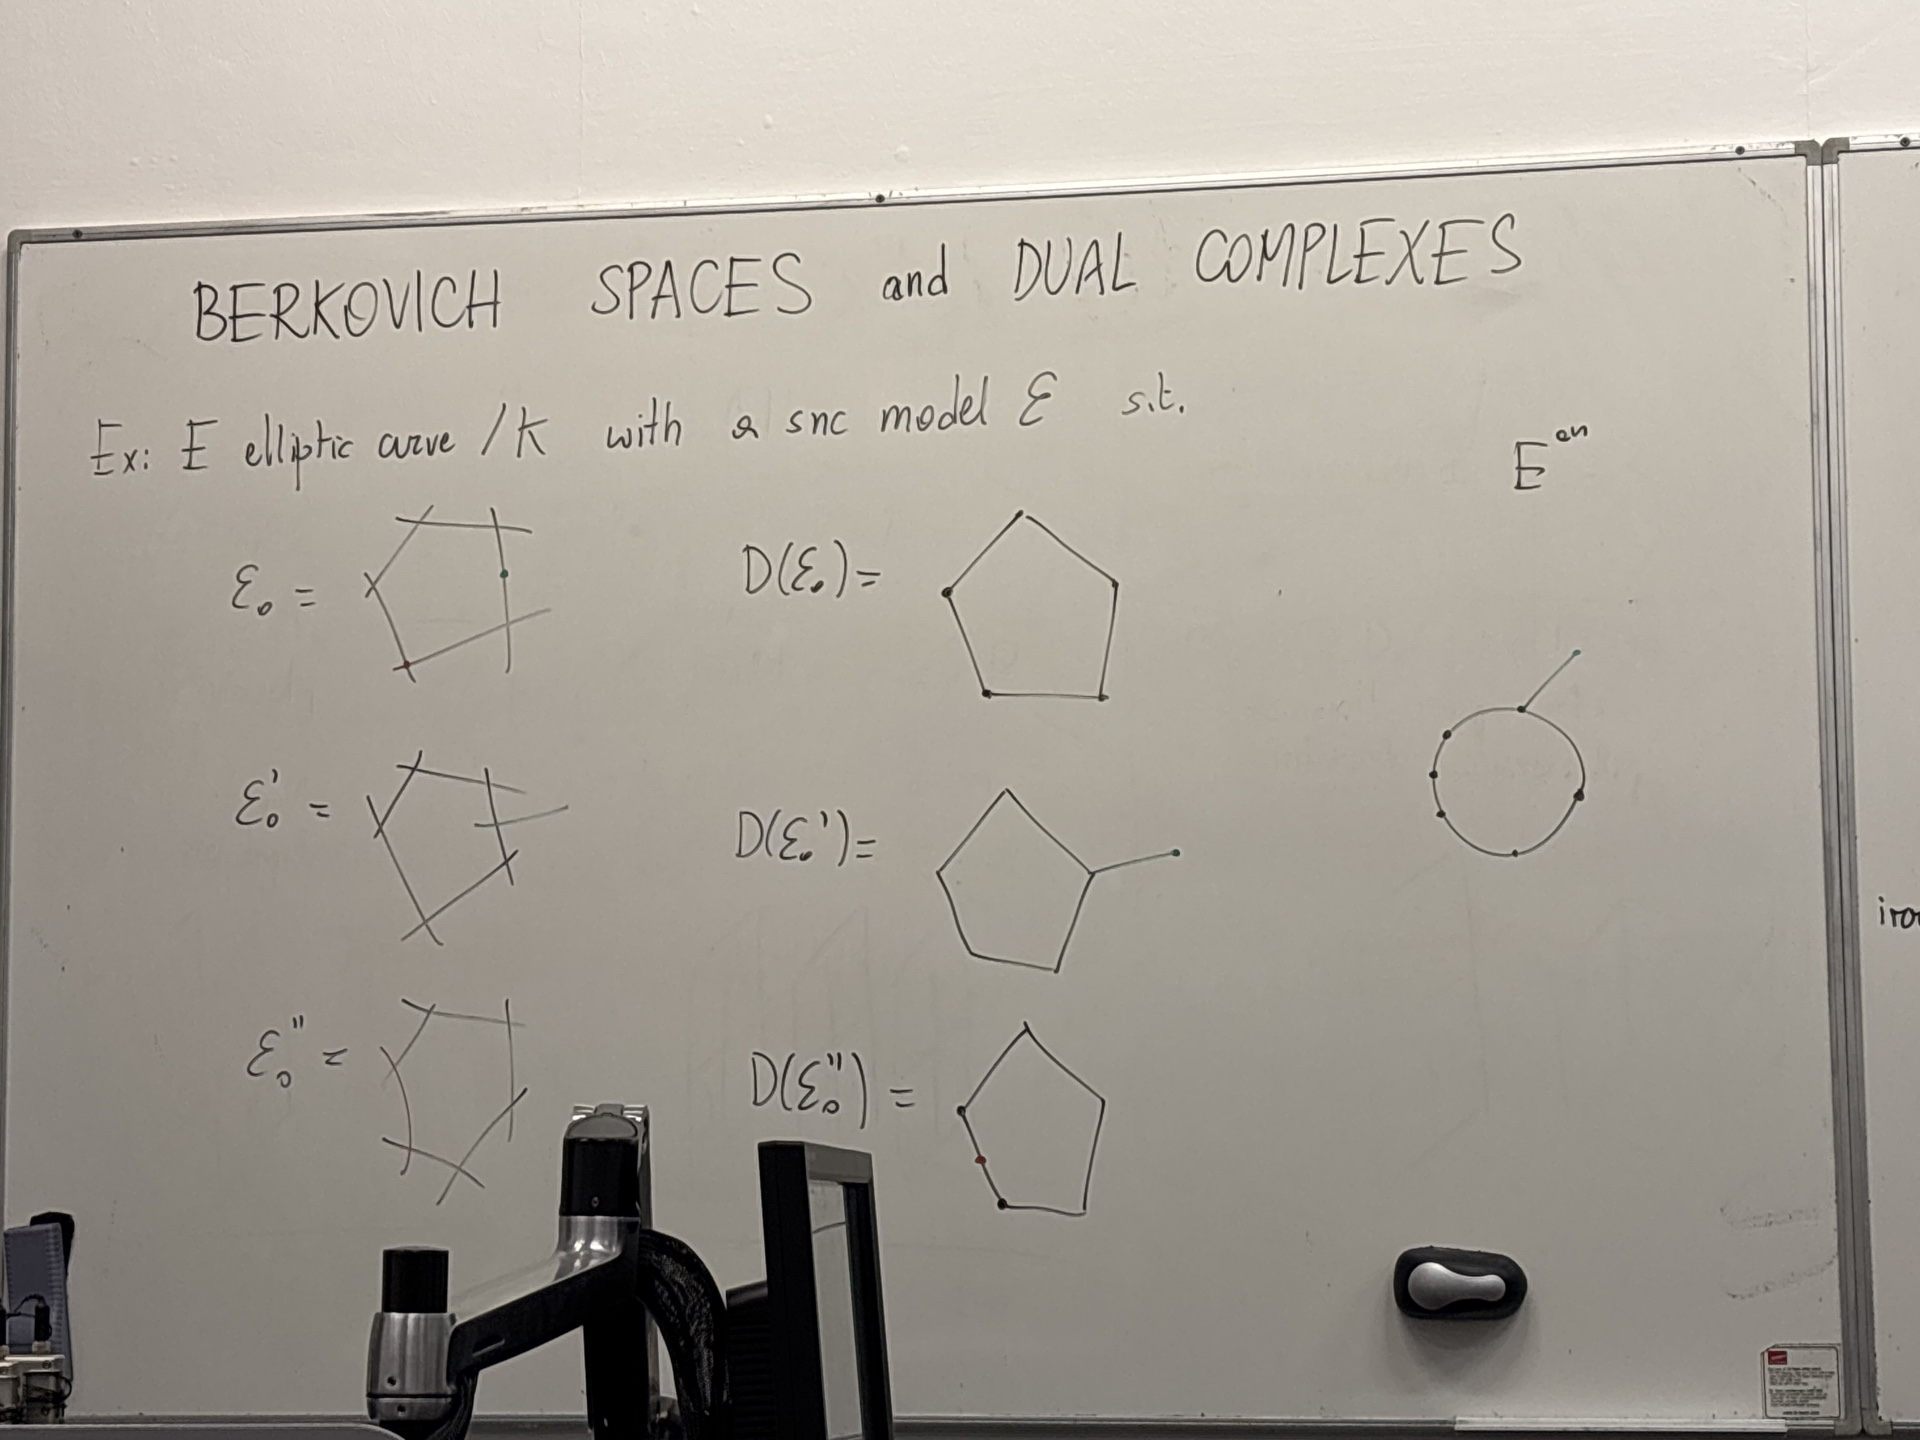
\includegraphics[width=0.5\textwidth]{images/elliptic-skeleton.jpeg}
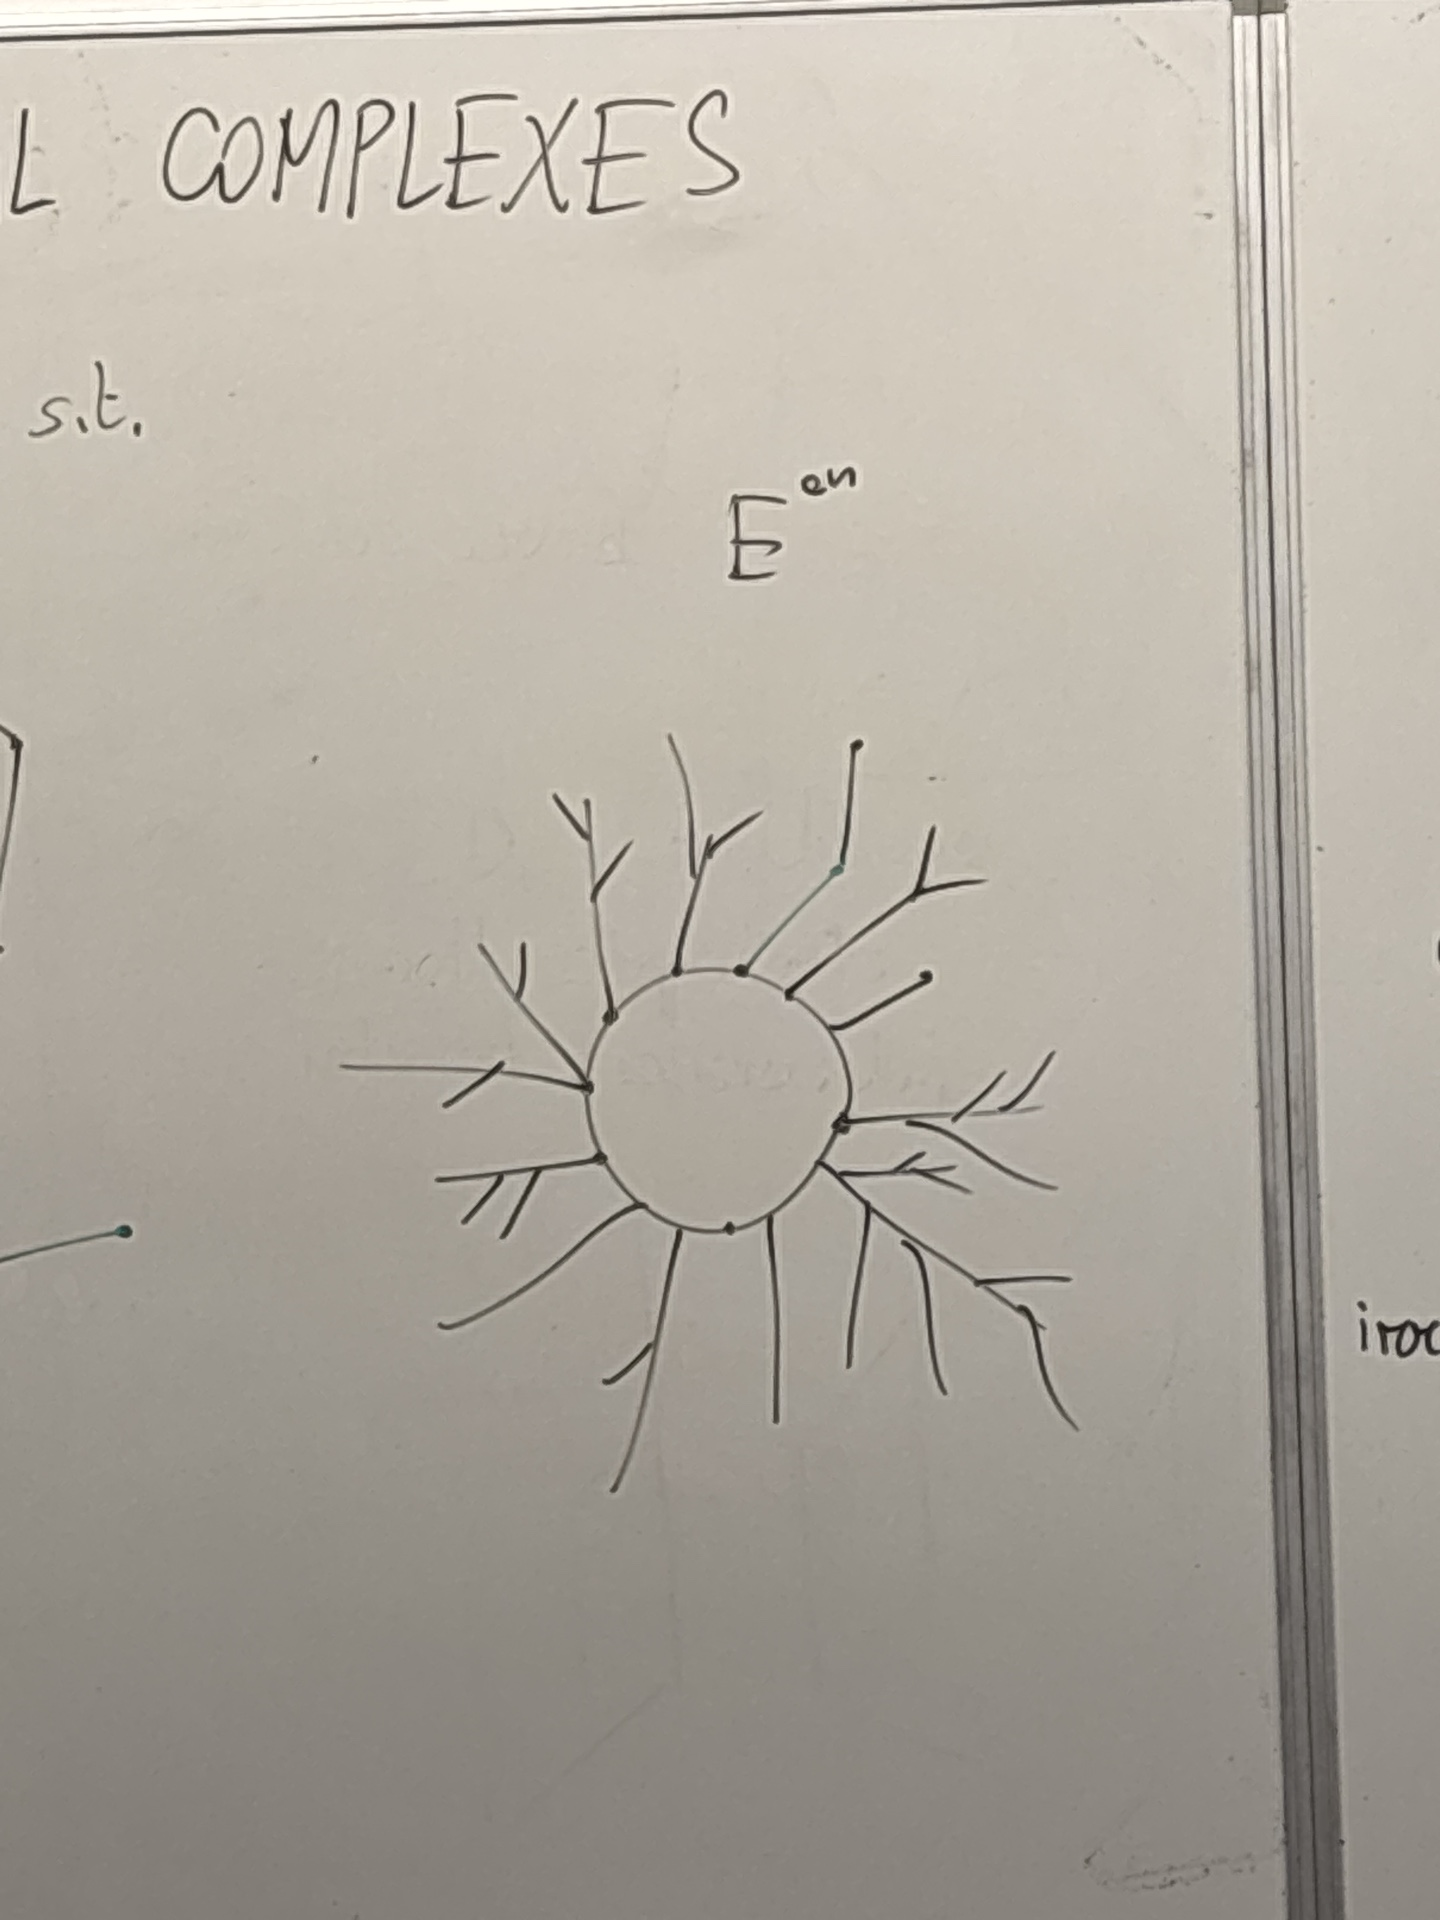
\includegraphics[width=0.5\textwidth]{images/elliptic-birkovich.jpeg}

Visual picture of how retraction works.

\section{Smooth projective CY setting}
Let \(X\) be a smooth projective \(CYn\) over \(K=\mathbb{C}(\!(t)\!)\). Also
assume there exists a family \(Y\to C\) over a smooth complex curve
\(C\), and \(X\) is the base change of \(Y\) to \(\mathbb{C}((t))\) a punctured
neighbourhood of some \(c\in C\). This is necessary for some arguments  which
require \(Y\) to be of finite type.

Can we pin down an snc model \((\mathcal{X},\mathcal{X}_0)\) such that the
skeleton of \(\mathcal{X}_0\) captures the essential geometry (i.e.\ every other
snc skeleton retracts? For elliptic curve this is pentagon with leg sticking out
for some reason).

Run MMP on \((\mathcal{X},\mathcal{X}_0)\) to get a minimal dlt pair
\(\mathcal{Y},\mathcal{Y}_0\). it is a fact that \(X\) has a projective good
minimal dlt model over \(R\), where we require that
\((\mathcal{Y},\mathcal{Y}_{0,\text{red}}\) is dlt. DLT ensures that the dual
complex of \(\mathcal{Y}_0\) can still be defined, it is the dual complex of
reduced \(\mathcal{Y}_0\).

minimal-- \(\mathcal{Y}_{0,\text{red}}\) is torsion.

good-- components of \(\mathcal{Y}_{0,\text{red}}\) are \(\mathbb{Q}\)--cartier.

[deFernex--Kollar--Xu] study behaviour of dual complex under MMP, and show that
\(D(\mathcal{Y}_0)\) is obtained from \(D(\mathcal{X}_0)\) using a sequence of
collapses.

[Kollar--Mori, deFernex--Kollar--Xu] The PL homeomorphism type of
\(D(\mathcal{Y}_0)\) is independent of choice of minimal dlt model
\(\mathcal{Y}\). Dual complexes of crepant birational models are PL
homeomorphic.

\begin{definition}
The essential skeleton \(Sk(X)\) is the image in \(X\an\) of the dual complex of
any minimal dlt model.
\end{definition}

Remarks-- you can take any snc model and any minimal dlt to define the skeleton.
The skeleton of a minimal DLT model sits inside the skeleton of any snc model.
``Which valuations inside \(X\an\) are essential?''

Alternatively [Kontsevich--Soibelman, Mustata--Nicaise] it is a union of
essential faces of \(Sk(\mathcal{X})\) or \(X\an\) corresponding to strata where
a canonical form \(\omega\)has minimal weight (discrepancy) in a suitable sense.

If haev a good minimal dlt model \(\mathcal{Y}\), then there is a retraction map
\(\rho_\mathcal{Y}: X\an\to Sk(X)\) that depends on \(\mathcal{Y}\). This is a
strong deformation retraction. In
particular \(X\an\) and \(Sk(X)\) have the same homotopy type.

Proposition (Nicaise--Xu) Sk(X) is a pseudomanifold with boundary, i.e.\ there
exists a triangulation in which \(Sk(X)\) is a union of equi-dimensional
\(m\)-simplices, every \((m-1)\)--simplex is a face of at most two
\(m\)--simplices, and any two \(m\)--simplices are connected by simple wall
crossing (strong connectedness).



Now consider \(X\) a maximally degenerate (i.e.\ Sk(X) is dim(X)--dimensional)
smooth projective CYn.
If \(n=1\) then the essential skeleton is \(\mathbb{S}^1\). If \(n=2\) then it
is \(\mathbb{S}^2\cong \mathbb{CP}^1\) by [Kulikov]. If \(X\) is strict
Calabi--Yau (i.e.\ \(\hh^{i,0}(X)=0\) for all \(0<i<n\)) then Nicaise--Xu show
that Sk(X) has \(\mathbb{Q}\)--homology of \(\mathbb{S}^n\). Dont know if it is
a sphere except in specific cases.

If \(X\) is hyperK\"ahler, then Sk(X) has rational homology of
\(\mathbb{CP}^{n/2}\) by [Jollar--Laza--Sacca--Voisin]. Dont know if it is
a projective space except in specific cases.

\subsection{Connection with mirror symmetry} Kotsevich--Soibelman think that the
retraction \(X\an\to \text{Sk}(X)\) is the non--archimedean analog of an SYZ
fibration \(X_t\to B\). Expect that the base manifold \(B\) is actually the
essential Skeleton.

[Nicaise--Xu--Yu] for any good minimal dlt model \(\mathcal{Y}\) of \(X\),
the retraction \(X\an\to Sk(X)\) is an affinoid torus fibration away from the
codimension \(2\) faces of \(Sk(X)\).

Affinoid torus fibration is tropicalisation map \((\mathbb{G}_m)^n\an\to \mathbb{R}^n\).

Theorem [Li] an syZ fibration exists on a large region \(U_t\subset X_t\) if a
non--archimedean conjecture holds. Thus the non--Archimedean picture has
concrete consequences on the `standard' SYZ picture. What's the
non--archimedean conjecture? Given a model \((\mathcal{Y},\mathcal{L})\) of
\((X,L)\), there is a distinguished function \(\phi\) on \(X\an\) which is a
solution to the non--Archimedean Monge--Ampere equation. Then the conjecture
says that there is a model \((\mathcal{Y},\mathcal{L})\) such that \(\phi =
\phi\circ \rho_\mathcal{Y}\) over the interior of the maximal faces of
\(Sk(X)\).




